\documentclass[12pt]{beamer}
\usepackage[utf8]{inputenc}
\usepackage[ngerman]{babel}
\usepackage{graphicx}
\usetheme{Boadilla}

\setbeamercovered{transparent}
\setbeamertemplate{navigation symbols}{}
\setbeamertemplate{footline}[frame number]
\setbeamertemplate{caption}[numbered]

\title{Atomphysik}
\author{\underline{Gruppe B14} \\ Daniel Wendland \\ Philipp Bremer \\ \textbf{Olexiy Fedorets} \\ Jonathan Hermann}
\date{\today}



%\mode<presentation>
%{
%	\usetheme{default}      % or try Darmstadt, Madrid, Warsaw, ...
%	\usecolortheme{default} % or try albatross, beaver, crane, ...
%	\usefonttheme{default}  % or try serif, structurebold, ...
%	\setbeamertemplate{footline}[frame number]
%	\setbeamertemplate{navigation symbols}{}
%	\setbeamertemplate{caption}[numbered]
%} 

%\usepackage{enumitem}
%
%\newlist{SubItemList}{itemize}{1}
%\setlist[SubItemList]{label={$-$}}
%
%\let\OldItem\item
%\newcommand{\SubItemStart}[1]{%
%	\let\item\SubItemEnd
%	\begin{SubItemList}[resume]%
%		\OldItem #1%
%	}
%	\newcommand{\SubItemMiddle}[1]{%
%		\OldItem #1%
%	}
%	\newcommand{\SubItemEnd}[1]{%
%	\end{SubItemList}%
%	\let\item\OldItem
%	\item #1%
%}
%\newcommand*{\SubItem}[1]{%
%	\let\SubItem\SubItemMiddle%
%	\SubItemStart{#1}%
%}%



\begin{document}


\begin{frame}[plain]
\titlepage
\end{frame}


\begin{frame}{Versuchsziele}
\Large
\begin{itemize}
\centering
	\item Verifizierung der $T^4$-Abhängigkeit im Stefan-Boltzmann Gesetz
	\item Bestimmung der Emissionskoeffizienten eines Leslie-Würfels
	\item Feststellung, welche Seite am ehesten einem schwarzen Strahler gleicht
\end{itemize}
\end{frame}


\begin{frame}{Gliederung}
\begin{enumerate}
	\Large
	\item{Theoretische Grundlagen}
	\item{Versuchsaufbau}
	\item{Versuchsdurchführung}
	\item{Kalibration}
		\begin{enumerate}
			\item $0^\circ C, 100^\circ C$
			\item Raumtemperatur $T_0$
		\end{enumerate}
	\item{Auswertung}
		\begin{enumerate}
			\item{lineare Regression an $T^4$}
			\item{Bestimmung der Emissionskoeffizienten}
			\item{Fit an $T^x$}
		\end{enumerate}
	\item{Fazit}
\end{enumerate}
\end{frame}

\begin{frame}{Theoretische Grundlagen}
\begin{itemize}
	\item{Plancksches Strahlungsgesetz}
	\begin{equation*}
	E_{\lambda,s}= 2 \cdot \pi \cdot \frac{h \cdot c^2}{\lambda^5} \cdot \frac{1}{e^{\frac{h\cdot c}{\lambda \cdot k \cdot T}}-1}
	\end{equation*}
	
	\item{Stefan-Boltzmann Gesetz}
	\begin{equation*}
	E_s(T)=\epsilon \cdot \sigma \cdot T^4,
	\qquad
	mit \;\; \sigma = 5.67 \cdot 10^{-8} \frac{W}{m^2K^4}
	\end{equation*}
	
	\item{Emissionskoeffizient}
	\begin{equation*} \label{eq:epsilon}
	\epsilon = \frac{P_{gemessen}}{P_{ideal}} = \frac{\frac{U_{gemessen} \cdot v}{c}}{A_{sender}\cdot \frac{A_{empf.}}{\pi r^2} \cdot \sigma \cdot (T_{messung}^4-T_0^4)}
	\end{equation*}
\end{itemize}
\end{frame}


\begin{frame}{Versuchsaufbau}
\begin{figure}[H]
	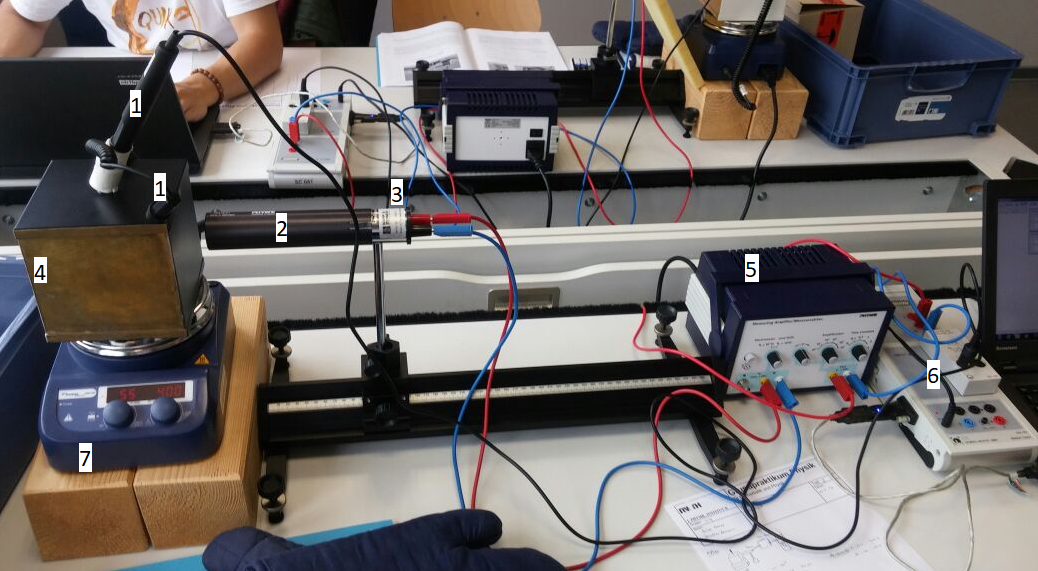
\includegraphics[scale=0.4]{../Protokoll/Bilder/Aufbau_markiert.png}
	\caption{Versuchsaufbau}
\end{figure}
\end{frame}

\begin{frame}{Versuchsdurchführung}
\begin{itemize}
	\item Messung der Umgebungstemperatur $T_0$ zu Beginn und am Ende des Versuchs
	\item Kalibration des Spannungsnullpunkts am Verstärker
	\item Füllen des Würfels mit Wasser, erhitzen auf $50^\circ C$
	\item Messung der Temperaturstrahlung aller Seiten in $5^\circ C$-Schritten
	\item Rauschmessung von Temperatur und Spannung
	\item Zwischen jeder Messung Thermosäule auf Wand richten und abschirmen
	\item Einstellungen am Sensor-CASSY:
	\begin{table}[h]
	\centering
	\begin{tabular}{cccc}
		\hline Messintervall & Messwertanzahl & Messzeit & U-Messbereich \\
		$50ms$& 125& $6.25s$& $-10V...+10V$ \\
		\hline
	\end{tabular}
	\end{table}
	
\end{itemize}
\end{frame}

\begin{frame}{Kalibration - $0^\circ C, 100^\circ C$}
\begin{itemize}
	\item Messung der Referenztemperatur in Eis- und kochendem Wasser
	\item Umrechnung der gemessenen Werte in reale mit
	\begin{equation*}
	T_{real} = m \cdot T_{gemessen} + n
	\end{equation*}
\end{itemize}
\begin{figure}[H]
	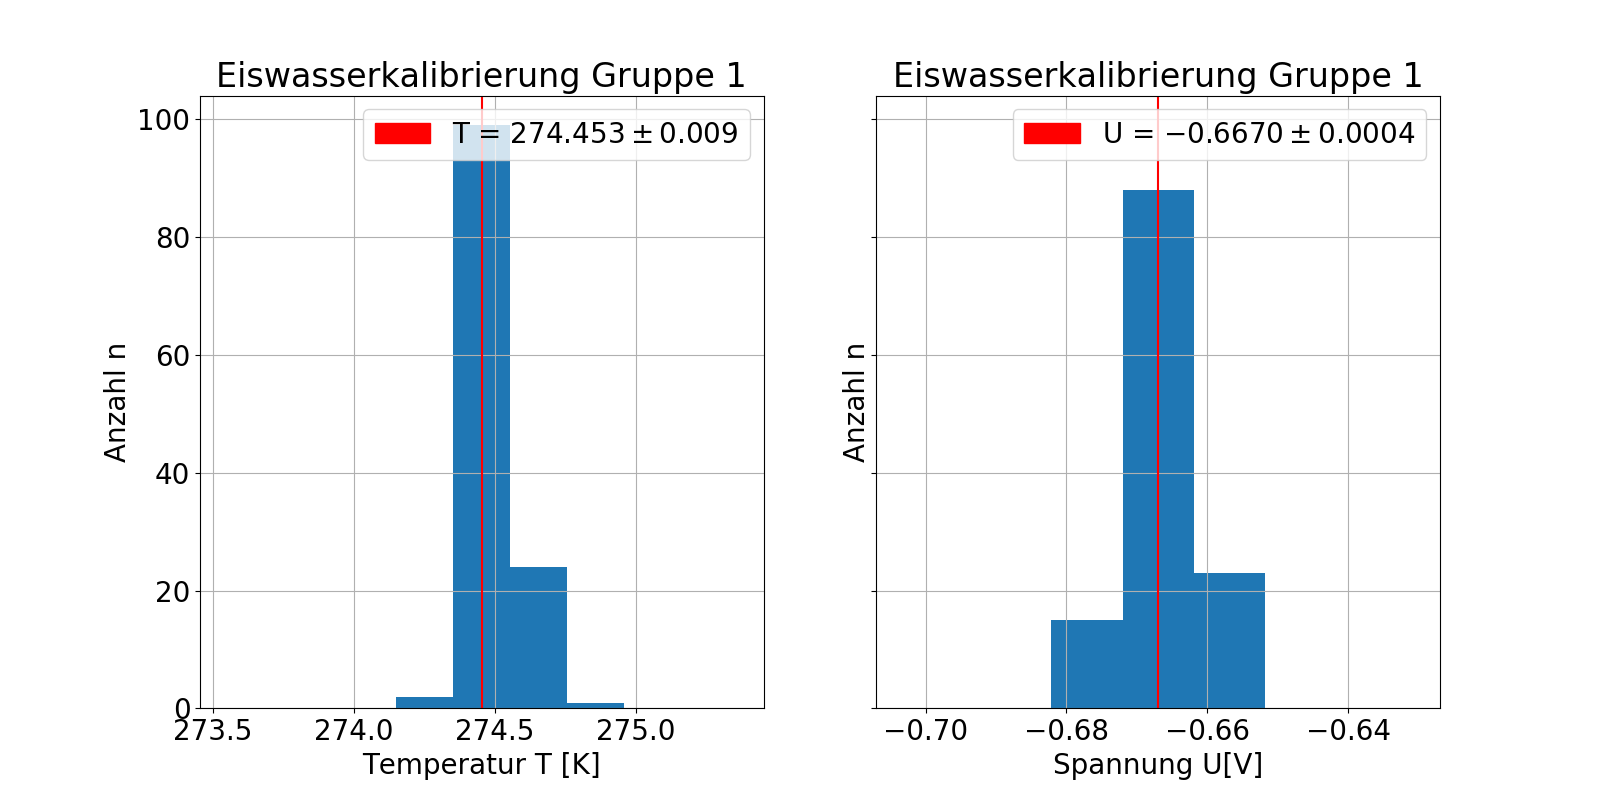
\includegraphics[scale=0.2]{../Protokoll/Bilder/Gruppe1_Eiswasser.png}
	\caption{$0^\circ C$-Kalibration der Gruppe 1}
\end{figure}
\end{frame}

\begin{frame}{Kalibration - $T_0$}
\begin{figure}[H]
	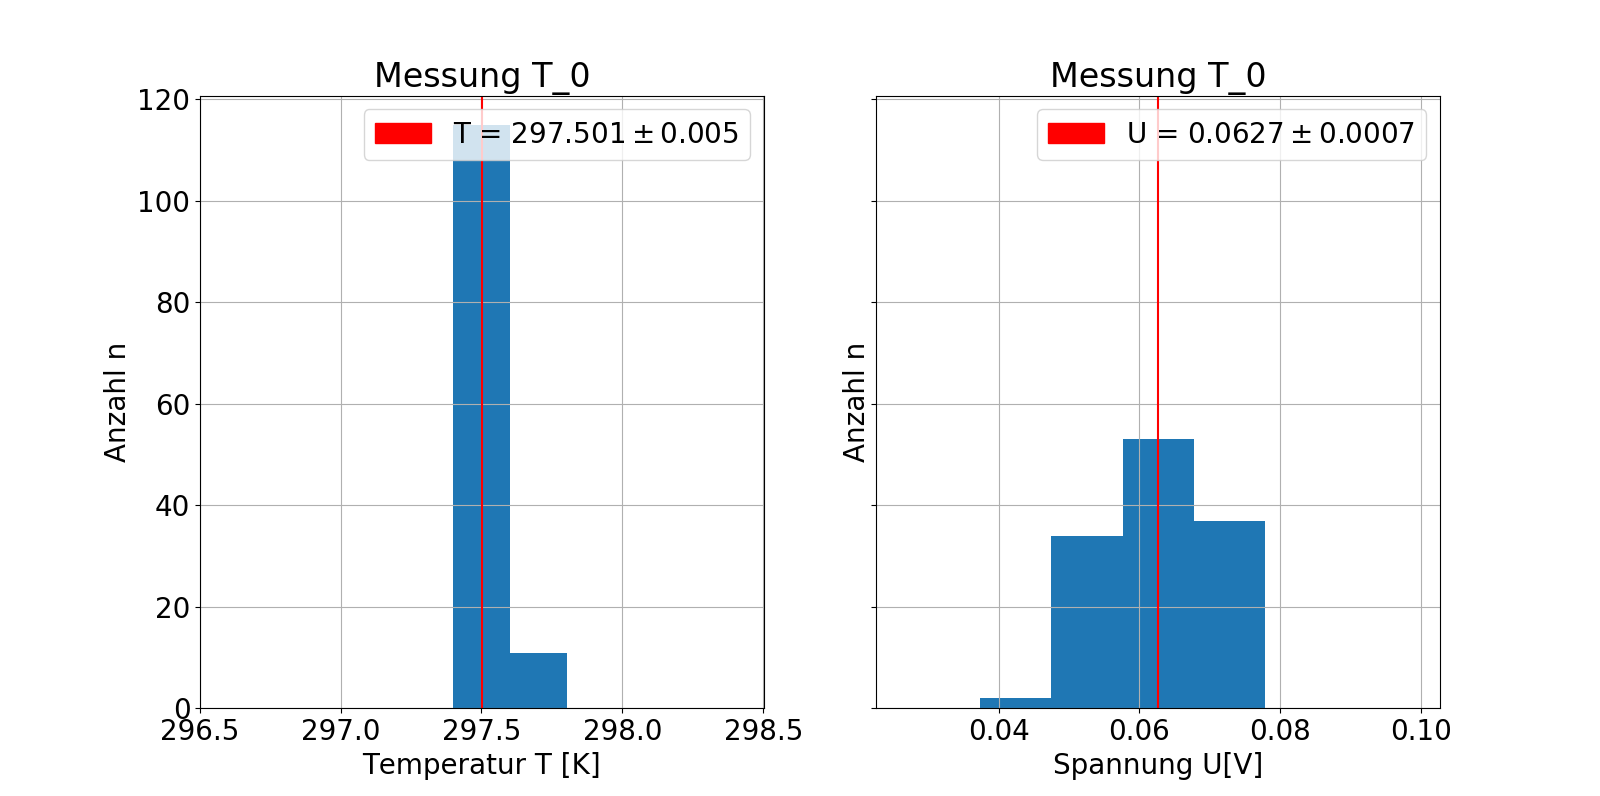
\includegraphics[scale=0.2]{../Protokoll/Bilder/Gruppe1_Zimmertemperatur.png}
	\caption{$T_0$-Kalibration der Gruppe 1}
\end{figure}
\begin{itemize}
	\item gemittelte Raumtemperatur:
	\begin{table}[h]
		\centering
		\begin{tabular}{cc}
			\hline Gruppe 1 & Gruppe 2\\
			$T_0= (297.501 \pm 0.005) K$ & $T_0= (298.053 \pm 0.006)K$\\
			\hline
		\end{tabular}
	\end{table}
\end{itemize}
\end{frame}


\begin{frame}{Auswertung - lin. Regression an $T^4$}
\begin{center}
$U(T) = a \cdot (T^4-T_0^4)+b$
\vskip -0.5cm
%\hskip -1cm
\begin{figure}[H]
	\centering
	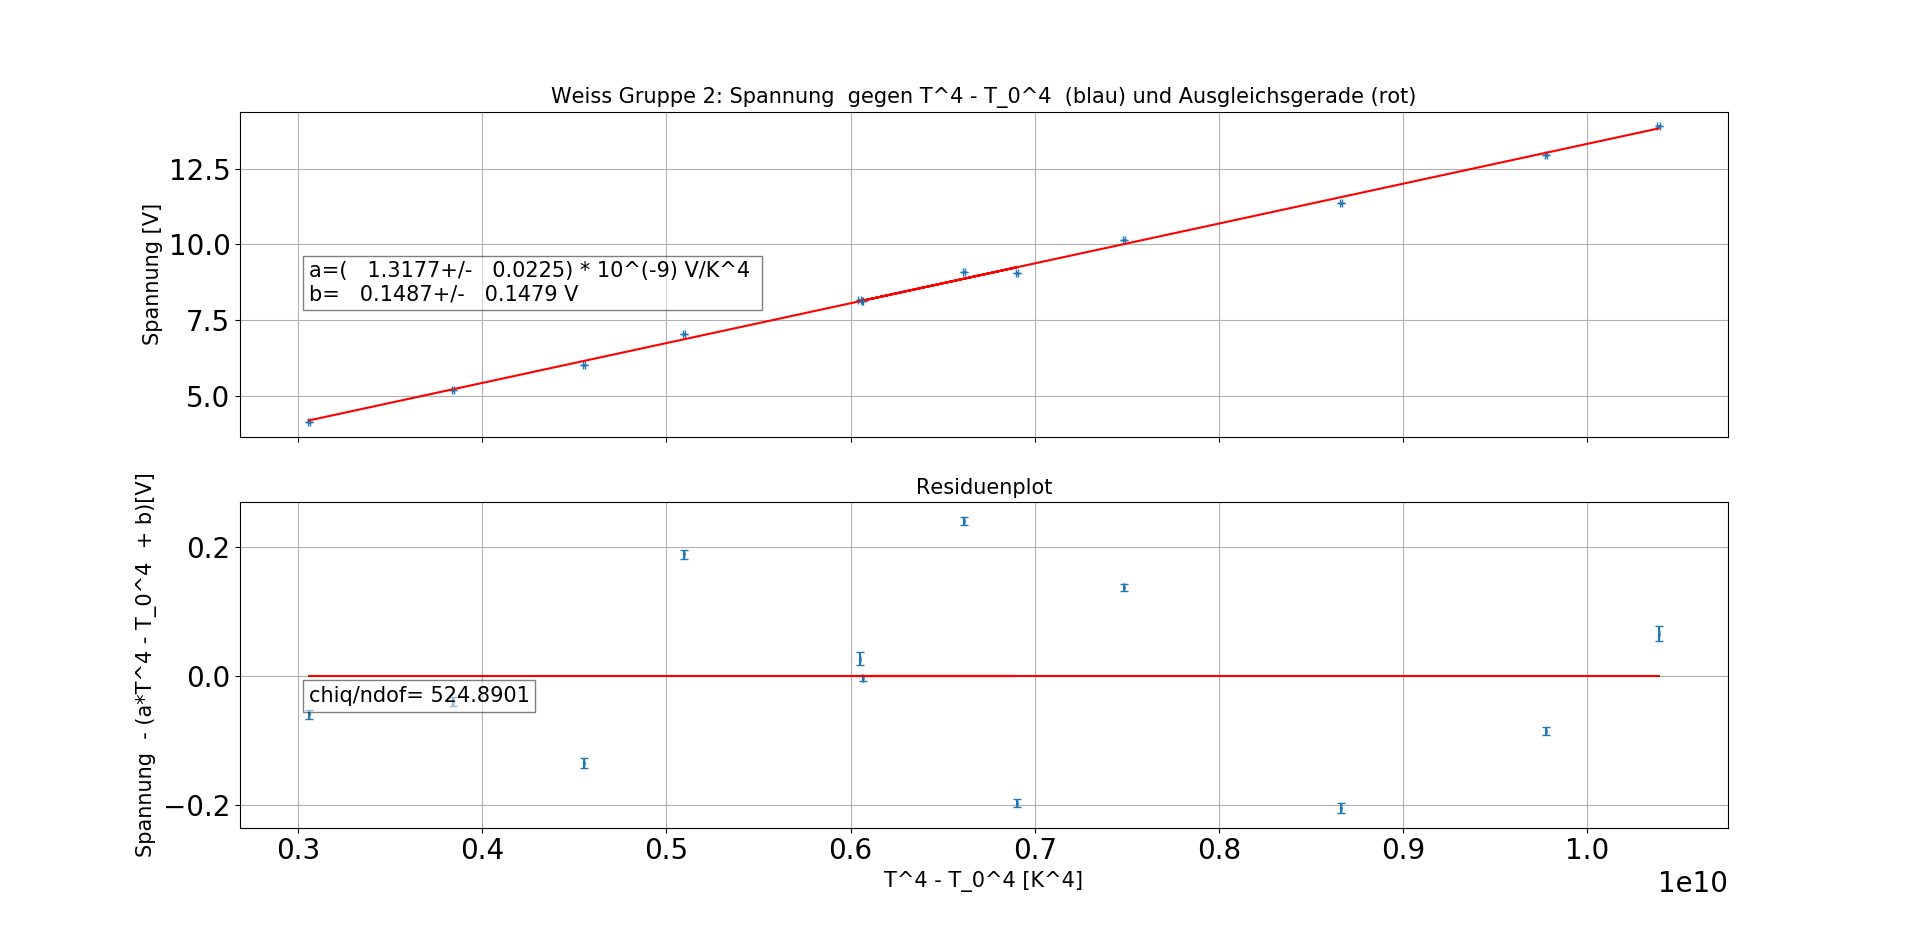
\includegraphics[scale=0.26]{../Protokoll/Bilder/Gruppe2_Weiss.png}
	\caption{$T^4$-Fit der Gruppe 2, weiße Seite}
\end{figure}

\end{center}
\end{frame}

\begin{frame}{Auswertung - Emissionskoeffizienten}
\vskip -0.5cm
\begin{equation*}
\epsilon = \frac{\frac{U \cdot v}{c}}{P_{ideal}} = a \cdot \frac{\pi \cdot r^2 \cdot v}{A_s \cdot A_e \cdot \sigma \cdot c}
\end{equation*}

\begin{equation*}
\sigma_{\epsilon,stat}=\frac{v r^2 \pi}{A_s A_e \sigma c}\cdot  \sigma_a \qquad
\sigma_{\epsilon ,sys}=\frac{a v r^2 \pi}{A_sA_e \sigma c^2}\cdot \sigma_c
\end{equation*}

\begin{table}
	\small
	\begin{tabular}{|c|c|c|}
	\hline Seite & Gruppe 1& Gruppe 2 \\
	\hline Schwarz& $\epsilon=0.905 \pm 0.005\pm 0.027$ &  $\epsilon=1.008 \pm  0.012 \pm 0.030 $\\
	\hline Weiß & $\epsilon=0.871 \pm 0.006\pm 0.026$ & $\epsilon= 0.965\pm 0.017 \pm 0.029$\\
	\hline Messing & $\epsilon=0.0602 \pm 0.0049\pm 0.0018$ & $\epsilon=0.0702 \pm 0.0023\pm 0.0021$\\
	\hline Spiegel & $\epsilon=0.0399 \pm 0.0016\pm 0.0012$ & $\epsilon=0.0442 \pm 0.0022\pm 0.0013$\\
	\hline  
	\end{tabular}
	\caption{Emissionskoeffizienten $\epsilon \pm \sigma_{stat} \pm \sigma_{sys}$}
\end{table}
\vskip -0.5cm
\begin{table}[h]
	\small
	\centering
	\begin{tabular}{|c|c|c|}
		\hline          & Seriennummer & Empfindlichkeit \\
		\hline Gruppe 1 & 120631 &$c_1=(0.160 \pm   0.0048)\frac{V}{W} $ \\
		\hline Gruppe 2 & 130815  &$c_2=(0.221 \pm   0.0066)\frac{V}{W} $\\
		\hline
	\end{tabular}
	\caption{Empfindlichkeiten der verwendeten Thermosäulen}
\end{table}

\end{frame}


\begin{frame}{Auswertung - Emissionskoeffizienten}

\begin{equation*}
\epsilon_{rel}=\frac{\epsilon_i}{\epsilon_{Schwarz}} 
\qquad
\sigma_{\epsilon_{rel}}=\sqrt{\left(\frac{\epsilon_i}{\epsilon_{Schwarz}^2} \cdot  \sigma_{\epsilon,Schwarz}\right) ^2 + \left( \frac{1}{\epsilon_{Schwarz}}\cdot \sigma_{\epsilon,i}\right) ^2}
\end{equation*}

\begin{table}[H]
	\small
	\hskip -0.3cm
	\begin{tabular}{|c|c|c|}
		\hline Relativwerte & Gruppe 1 & Gruppe 2\\
		\hline Weiß & $\epsilon_{rel}=0.956 \pm 0.011 \pm 0.041 $ & $\epsilon_{rel}=0.957 \pm 0.020 \pm 0.040$\\
		\hline Messing & $\epsilon_{rel}=0.069 \pm 0.005 \pm 0.030$ & $\epsilon_{rel}= 0.070\pm 0.012 \pm 0.030$\\
		\hline Spiegel & $\epsilon_{rel}=0.044 \pm 0.005 \pm 0.030$ & $\epsilon_{rel}= 0.044\pm 0.012 \pm 0.030$\\
		\hline  
	\end{tabular}
	\caption{Relativwerte der Emissionskoeffizienten}
	\label{table:EpsilonRel}
\end{table}

\end{frame}


\begin{frame}{Auswertung - Fit an $T^x$}
\begin{center}
	\vskip -1cm
	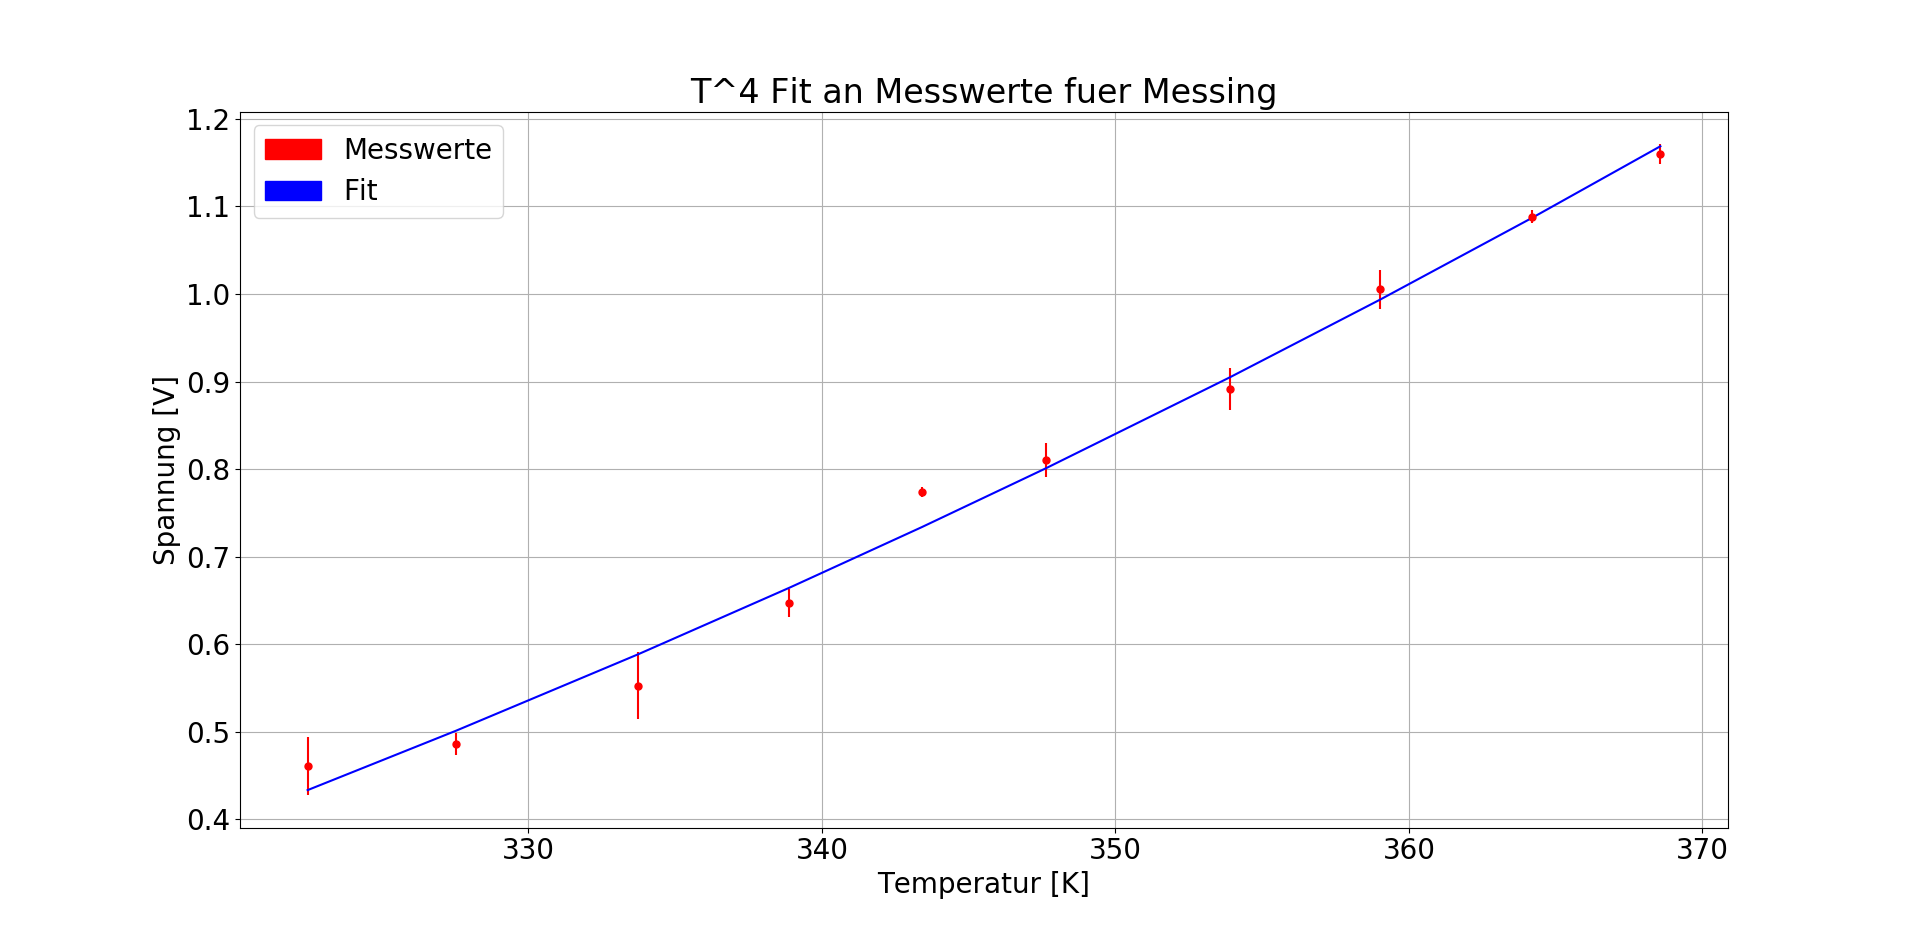
\includegraphics[scale=0.25]{../Protokoll/Bilder/Gruppe2_Fit_Messing.png}
\end{center}
\vskip -1cm
\begin{table}[H]
	\small
	\centering
	\begin{tabular}{|c|c|c|c|}
		\hline $ U=p_0+p_1\cdot T^{p_2}$& $p_0$& $p_1$ & $p_2$\\
		\hline Gruppe 1 / Weiß & $(-7.0 \pm 1.5)V $ & $ (1.5 \pm 4.4  )\cdot 10^{-9}\frac{V}{K^4}$  & $ 3.9\pm 0.5 $ \\
		\hline Gruppe 2 / Messing &  $(-0.7 \pm 0.7)V $ & $ (0.4 \pm 4.3  )\cdot 10^{-9}\frac{V}{K^4}$  & $ 3.8\pm 1.9 $  \\
		\hline
	\end{tabular}
\end{table}
\end{frame}

\begin{frame}{Auswertung - Fazit}
\begin{itemize}
	\item Zusammenhang des Stefan-Boltzmann Gesetzes konnte bestätigt werden, $\chi^2/ndf$ sind allerdings zu groß aufgrund von zu kleinen Fehlern
	\item Fehler auf Emissionskoeffizenten wahrscheinlich zu klein, Werte der Gruppe 2 für schwarz und weiß sind unrealistisch
	\item Schwarze Seite gleicht wie erwartet am ehesten einem schwarzen Strahler
	\item 4er-Potenz im Stefan-Boltzmann Gesetz konnte annähernd bestätigt werden (aber mit hoher relativer Unsicherheit)
\end{itemize}
\end{frame}

%\begin{frame}
%\frametitle{Versuchsaufbau}
%\begin{figure}[h]
%\begin{center}
%\includegraphics[width=7cm]{Versuchsaufbau.JPG}
%\caption{Versuchsaufbau, Quelle: Praktikumsskript}
%\end{center}
%\end{figure}
%\end{frame}
%
%\begin{frame}
%\frametitle{Versuchsdurchführung}
%\begin{itemize}
%\item{Vorbereitung: Rauschmessungen (Kalibration), Umgebungstemperatur}
%\item{Messablauf: Wunschseite zur Thermosäule drehen, warten Spannung stabilisiert}
%\item{Möglicherweise Messbereich erhöhen}
%\item{Messablauf in $5^\circ$C Schritten wiederholen von $50^\circ$C- $95^\circ$C }
%\end{itemize}
%\end{frame}
%
%
%\begin{frame}
%\frametitle{Auswertung}
%
%\begin{figure}[h]
%\begin{center}
%\includegraphics[width=6cm]{Eiswasser1.png}
%\includegraphics[width=6cm]{Siede1.png}
%\caption{Rauschmessung mit Eiswasser und Siedewasser für Gruppe 1}
%\label{Eisrauschen}
%\end{center}
%\end{figure}
%\end{frame}
%
%\begin{frame}
%\frametitle{Fehlerrechnung}
%\begin{align}
%&T_{gem.}=\frac{1}{N}\sum\limits_{i=1}^N T_i\\
%&\sigma_{T_{gem.}}=\sqrt[]{\sum\limits_{i=1}^N \frac{(T_i-T_{gem.})^2}{N(N-1)}} \\
%\end{align}
%\end{frame}
%
%
%\begin{frame}
%\frametitle{Temperaturkalibrierung}
%\begin{align}
%T_{real}=a\cdot T_{gem.} + b
%\end{align}
%
%\begin{figure}[h]
%\begin{center}
%\includegraphics[width=7cm]{KalibrierungG1.png}
%\caption{Erwartete Temperatur gegen gemessene Temperatur zur Korrektur der aufgenommen Daten}
%\end{center}
%\end{figure}
%\end{frame}
%
%\begin{frame}
%\begin{figure}[h]
%\begin{center}
%\includegraphics[width=8.5cm]{lineare_regression_weiss1.png} 
%\caption{Lineare Anpassung der Form $U(T) = a \cdot (T_{real}^4 -T_0^4) +b$ an die Messwerte der weißen Würfelseite, Gruppe 1}
%\end{center}
%\end{figure}
%\end{frame}
%
%\begin{frame}
%\begin{figure}[h]
%\begin{center}
%\includegraphics[width=8.5cm]{residuenplot_weiss1.png}
%\caption{Zugehöriger Residuen der Messwerte der weißen Würfelseite, Gruppe 1}
%\end{center}
%\end{figure}
%\end{frame}
%
%\begin{frame}
%\begin{figure}[h]
%\begin{center}
%\includegraphics[width=6cm]{Tfitmessing2.pdf} 
%\includegraphics[width=6cm]{TFitMessingres2.pdf}
%\caption{Nichtlineare Anpassung an die Messwerte der Messingseite des Würfels, Gruppe 2}
%\label{tx}
%\end{center}
%\end{figure}
%\begin{equation}
%U(T) = p_0+p_1(T^{P_2}-T_0^4)
%\label{lol}
%\end{equation}
%\end{frame}
%
%
%\begin{frame}
%\frametitle{Emissionskoeffizient}
%\begin{itemize}
%\item  \begin{equation}
%P_{gem.} = \frac{U_{gem.}}{c \cdot 10^4}
%\end{equation}
%\item c Empfindlichkeit der Thermsäule
%\end{itemize}
%Daraus folgt :
%\begin{equation}
%\Rightarrow\epsilon = \frac{P_{gem.}}{P_{ideal}} = \frac{\frac{U_{gem.}}{c \cdot 10^4}}{A_s A_e \frac{\sigma}{r^2 \pi} (T_{gem.}^4 - T_0^4)}
%\end{equation}
%\end{frame}
%
%\begin{frame}
%\frametitle{Emissionskoeffizient}
%\begin{equation}
%\epsilon = \frac{P_{gem.}}{P_{ideal}} = \frac{\frac{U_{gem.}}{c \cdot 10^4}}{A_s A_e \frac{\sigma}{r^2 \pi} (T_{gem.}^4 - T_0^4)}
%\end{equation}
%
%\begin{align}
%\rightarrow\sigma_{\epsilon} = \epsilon \ \sqrt[]{(\frac{\sigma_a}{a})^2 + (0,03)^2}
%\end{align}
%\end{frame}
%
%\begin{frame}
%\begin{table}[h]
%\centering
%\begin{tabular}{|c|c|c|c|c|} \hline
%& Silber & Messing & Weiß & Schwarz  \\ \hline
%$\epsilon$ &$0.046\pm0.004$  &$0.110\pm0.005$  &$0.906\pm0.028$  &$0.924\pm0.029$  \\ \hline
%\end{tabular}
%
%\caption{Gruppe 1 Emissionskoeffizienten für die vier Seiten des Lesliewürfels}
%\begin{tabular}{|c|c|c|c|c|} \hline
%& Silber & Messing & Weiß & Schwarz  \\ \hline
%$\epsilon$ &$0.069\pm0.005$  &$0.100\pm0.007$  &$0.921\pm0.029$  &$0.950\pm0.030$   \\ \hline
%\end{tabular}
%
%\caption{Gruppe 2 Emissionskoeffizienten für die vier Seiten des Lesliewürfels}
%\end{table}
%\end{frame}
%
%


\end{document}
